\documentclass[conference, a4paper]{IEEEtran}

\usepackage{graphicx}

% used for flow charts
\usepackage{pgf}
\usepackage{tikz}
\usepackage{tikz-qtree}
\usepackage{reotex}

% package url is used when citing a website
\usepackage{url}

\usepackage{amssymb}
\usepackage{amsmath}
\usepackage{cite}
\usepackage[normalem]{ulem}
% for a smile-face character
\usepackage{wasysym}
% listing for codes
\usepackage{listings}
% listing for golang
% NOTE listings-golang.sty is required
\usepackage{listings-golang}
% to support flow graphs
\usepackage{textcomp}
% highlight in tables
\usepackage{xcolor}
\usepackage{colortbl}
% used to encode algorithms
\usepackage[linesnumbered, ruled, vlined]{algorithm2e}
\usepackage{array}

% positioning is used for below lef = of
\usetikzlibrary{shapes,shadows,arrows,automata,positioning}
% some tikz-styles on reo channels, not required in papers that have nothing to do with Reo

% finally no todos should exist in this draft
\usepackage[textsize=tiny]{todonotes}
\usepackage{xcolor}
\newcommand{\liyi}[1]{\textcolor{red}{Liyi: {#1}}}

% -------------------------------------- configurations -----------------------------------------
% declaration of environments
\newtheorem{theorem}{Theorem}
\newtheorem{definition}{Definition}
\newtheorem{example}{Example}

% personal characters
\newcommand{\rblock}[0]{\circleddash}
\newcommand{\rread}[0]{\rhd}
\newcommand{\rnoread}[0]{\otimes}
\newcommand{\smap}[1]{[{#1}]}
\newcommand{\rempty}[0]{\varnothing}

\newcommand{\OUT}[0]{\mbox{OUT}}
\newcommand{\IN}[0]{\mbox{IN}}

% style of source code environment listings
\lstset{basicstyle=\footnotesize\ttfamily,breaklines=true, frame=shadowbox}
\lstset{numbers=left}
\lstset{xleftmargin=2em, xrightmargin=2em}
\lstset{language=Golang}

% --------------------------------------- information -------------------------------------------
\title{Active Learning from Blackbox to Timed Connectors}
\author{
\IEEEauthorblockN{Yi Li, Meng Sun and Yiwu Wang}
\IEEEauthorblockA{
LMAM \& Department of Informatics, School of Mathematical Sciences, Peking University,
Beijing, China\\
liyi\_math@pku.edu.cn, summeng@math.pku.edu.cn, yiwuwang@126.com
}
}

\begin{document}
\maketitle 
\begin{abstract}
  Coordination models and languages play a key role in formally specifying the communication and
  interaction among different components in large-scale concurrent systems. In this
  paper, we use active learning to extract timed connector models from black-box
  system implementation. 
  Firstly, parameterized Mealy machines(PMM) is introduced as an operational semantic
  model for channel-based coordination language Reo. With product and link operators defined, we can
  construct complex connectors by joining basic channels in form of PMM. Moreover, with a
  concretize mapping function, PMMs can be easily transformed into Mealy machines, and the latter can be
  extracted by an optimized L* algorithm.
\end{abstract}

\begin{IEEEkeywords}
  Active Learning, Coordination, Connectors
\end{IEEEkeywords}

\section{Introduction} 

Distributed real-time embedded systems (DRES) are reforming our lives with the
Internet of Things(IoT), wherein individual components are composed via \emph{connectors} 
to build complex systems. 
%Such systems could be distributed logically or physically, which
%makes coordination processes even more complicated. 
In this case, we need to specify the coordination
processes with \emph{coordination languages}, such that formal techniques can be applied to
guarantee their reliability.

As a real-time extension of \emph{Reo}, \emph{Timed
Reo}\cite{DBLP:conf/sefm/ArbabBBR04,DBLP:conf/tase/Meng12} is used in this paper to formalize
connectors in DRES. 
Reo is a channel based exogenous coordination language proposed by F. Arbab in
\cite{DBLP:journals/mscs/Arbab04}, which is a powerful ``glue language'' in component-based
development\cite{DBLP:journals/sigsoft/Gill03}. 
\begin{figure}[ht]
  \begin{center}
    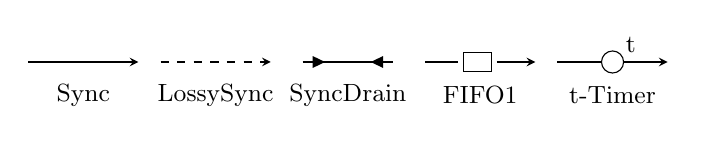
\begin{tikzpicture}[scale=1.4]

\tikzstyle{every node}=[font=\small]
\tikzstyle{label}=[draw=none]

\draw (0.5, -0.3) node[label] {Sync};
\draw (1.7, -0.3) node[label] {LossySync};
\draw (2.9, -0.3) node[label] {SyncDrain};
\draw (4.1, -0.3) node[label] {FIFO1};
\draw (5.3, -0.3) node[label] {t-Timer};

\sync{(0,0)}{(1,0)}{}
\lossysync{(1.2,0)}{(2.2,0)}{}
\syncdrain{(2.4,0)}{(3.4,0)}{}
\fifoe{(3.6,0)}{(4.6,0)}{}

\timer{(4.8,0)}{(5.8,0)}{node [above left] {t}}

\end{tikzpicture}

  \end{center}
  \caption{Basic Reo Channels}
  \label{fig:basic}
\end{figure}

Formal verification and validation techniques have also been proved applicable for timed connectors
\cite{DBLP:conf/tase/LiCWS15,DBLP:journals/scp/Kemper12} 
However, most of these tools heavily rely on manually modelling.
\emph{Correctness} of connectors is closely related to some low-level implementation details.
For example, well-written code may behave dramatically weird with an improper set of concurrency
primitives. Such scenarios happen frequently in embedded systems with different hardware platforms or
operating systems. Consequently, manually extracting a proper model from an existing connector
implementation seems rather unreliable, even with reference to its source code.

In this paper we address this question by means of active learning
\cite{DBLP:journals/iandc/Angluin87, DBLP:conf/fase/RaffeltS06}.
First of all, we introduce \emph{parameterized Mealy machine} as a parameterized
semantics for timed Reo, which can be transformed to concrete Mealy machines with a
specified alphabet. Then the $L*$ algorithm \cite{DBLP:journals/iandc/Angluin87} is adapted and
optimized to extract Mealy machines with timed action from the connector implementations as
blackboxes. 

The rest of the paper is organized as follows: In Section \ref{sec:semantics}, we defines an
operational semantics of Reo, which is used in Section \ref{sec:activelearning} to show how to
extract Reo models from blackboxes by means of active learning. In Section
\ref{sec:experiment}, we discuss the implementation and optimization of the approach. 
Finally, Section VI concludes the paper. Due to the limit of space, many technical details are
omitted in this paper.
Please refer to \cite{reo-learn-github} for further contents.


\section{Timed Connectors as Mealy Machines}
\label{sec:semantics}

In this section, we introduce PMM as an intermediate form to transform timed connectors into
Mealy machines with timed action. In this paper, we assume that time dimension is defined on the
national number $\mathbb{Q}$, which is generally as expressive as $\mathbb{R}$ and much easier to
formalize\cite{DBLP:journals/fmsd/PrabhakarDM015}. Since connectors contain only finite number of
channels, we can always find a minimal time unit (denoted as $T$) where real-time connectors can be
discretized.

%\subsection{Time Domain}
%Time has been investigated in several extensions of Reo. For example, timed
%Reo\cite{DBLP:conf/sefm/ArbabBBR04, DBLP:conf/fmoods/MengA07}, hybrid Reo\cite{DBLP:conf/icfem/ChenSS14}, etc.
%Generally, these models are designed to handle real-time behavior where time is defined on the
%real number field $\mathbb{R}$. However, there are also some works like
%\cite{DBLP:journals/fmsd/PrabhakarDM015} where
%rational time indeed  makes things easier. In this paper, we choose the rational number field
%$\mathbb{Q}$ as our time domain, which simplifies discretization of timed behavior greatly.

%As presented in section \ref{sec:reo}, all real-time behavior in timed Reo comes with a finite set
%of timed channels. We use
%$t_i\in\mathbb{Q}, i=1,2,\dots,n$ to denote the delays of these timed channels, and then we can define a precision
%function $prec$ which calculate a gcd-style \emph{maximal time precision}:
%\[
%prec(t_1,\dots,t_n) = \max\{T\in\mathbb{Q}|\forall t_i.\exists n_i\in\mathbb{N}.t_i=n_i\cdot T\}
%\]
%It's easy to prove that such a $T$ always exists.

%In embedded systems, the maximal time precision is also called ``clock-period'', which is the basic
%time unit provided by an oscillator. For example, a widely-used Intel-80C51 microcontroller works
%under the frequency 16Mhz, where the clock-period is $62.5$ns. A reasonable assumption comes that
%such a maximal time precision $dt=prec(t_1,\dots,t_n)$ should always be provided to make sure
%different components are able to work together. Then all $t_i$-Timers can be seen as $n_idt$-Timers
%for some $n_i$ and we use $n_i$-Timers instead in the following sections.

%Besides, we add a timed action ``$T$'' in Mealy machines. It indicates that the corresponding
%transition will take one time unit to finish.

\subsection{Parameterized Mealy Machine}
In this work, we use \emph{Mealy machines} to model Reo connectors.
Mealy machine is an extension of finite state machine to model reactive systems.
Following its definition in \cite{DBLP:conf/sfm/SteffenHM11}, we present a model here named
\emph{parameterized Mealy machine} to formalize timed connectors.

\begin{definition}[Parameterized Mealy Machine]
  A \emph{Parameterized Mealy Machine} with a parameter $\Sigma$ is defined as a 6-tuple
  $\mathcal{PM}=\langle S, s_0, I, O, \delta, \lambda\rangle$ where 
  \begin{itemize}
    \item[-] The value of $\Sigma$ is a \emph{finite} data set (hereinafter referred as
      alphabet), e.g.  $\{a,b\}$,
    \item[-] $S$ maps an alphabet to a \emph{finite} set of states,
    \item[-] $s_0$ is the initial state. It satisfies $\forall \Sigma.s_0\in S(\Sigma)$,
    \item[-] $I$ is a finite set of source-ends,
    \item[-] $O$ is a finite set of sink-ends,
    \item[-] $\delta$ maps an alphabet to an \emph{output function}. We use
      $\delta(\Sigma):S(\Sigma)\times Input(\Sigma,I,O)\rightarrow Output(\Sigma,O)$ to denote the
      output function,
    \item[-] $\lambda$ maps an alphabet to a \emph{transition function}. We use
      $\lambda(\Sigma):S(\Sigma)\times Input(\Sigma,I,O)\rightarrow S(\Sigma)$ to denote the
      transition function.
  \end{itemize}
\end{definition}

In the definition above, \emph{Input} and \emph{Output} are used to generate the set of input actions
and output actions from the corresponding alphabets and source/sink ends. $Input(\Sigma,I,O)$ is
defined as the intersection of the set of input events $Evt_{in}$ and an additional \emph{time
action} T. Here every $in\in Evt_{in}$ is an evaluation on both sink and source ends and
\[
\forall i\in I.in(i)\in\Sigma\cup\{\rempty\}\land \forall o\in O.in(o)\in\{\rnoread, \rread\}
\]
where we use $\bot$ to indicate that there is \emph{no} data item on a channel end. 
Besides, $\rread$ means that a sink end is ready for writing, $\rnoread$ otherwise. 
In the same way,
$Output(\Sigma,O)$ is defined as a set of output events in form of evaluations on $O$, with an
additional symbol $\rblock$ indicating an input failure.

%A non-timed input action $a\in Input(\Sigma,I,O)$ can be restricted to $I'\subseteq I$, denoted by
%$a\downarrow_{I'}$ which is defined on $Input(\Sigma,I',O)$ and satisfies
%\[
%\forall i\in I'. a\downarrow_{I'}(i)=a(i)
%\]
%Restriction on output actions can be defined similarly.

\begin{example}[Input and Output]
  If we have a simple alphabet with only one item $d_0$, a source-end named $A$, and a
  sink-end named $B$, the input actions would be
  \begin{eqnarray*}
    & & Input(\{d_0\},\{A\},\{B\}) \\
    & = & \{\{A\mapsto d_0,B\mapsto\rread\},\{A\mapsto d_0,B\mapsto\rnoread\}, \\
    & & \{A\mapsto\bot,B\mapsto\rread\}, \{A\mapsto\bot,B\mapsto\rnoread\},T\}
  \end{eqnarray*}
  and its output actions
  \[
  Output(\{d_0\},\{A\},\{B\}) =\{\{B\mapsto d_0\},\varnothing, \rblock\}
  \]
\end{example}

We use $\varnothing$ to denote the empty output when no data item is written to any sink end.
For example, in the above case $\varnothing$ is used to denote $\{B\mapsto\bot\}$.

Parameterized Mealy machines can be seen as an abstraction of Mealy machines, hence we
still need a convert function between the two models.

\begin{definition}[Concretize Mapping]
  We use $\smap{\mathcal{PM}}_{\Sigma}$ to denote the concrete Mealy machine which is determined by
  an abstract parameterized Mealy machine $\mathcal{PM}$ and the alphabet $\Sigma$. Apparently
  $\smap{\mathcal{PM}}_{\Sigma}$ can be described as
  \begin{eqnarray*}
    \smap{\mathcal{PM}}_{\Sigma} &=& 
    \langle
    \mathcal{PM}.S(\Sigma), \mathcal{PM}.s_0, \\
    & & Input(\Sigma, \mathcal{PM}.I, \mathcal{PM}.O), Output(\Sigma, \mathcal{PM}.O), \\
    & & \mathcal{PM}.\delta(\Sigma), \mathcal{PM}.\lambda(\Sigma),
    \rangle
  \end{eqnarray*}
\end{definition}

Now we can use PMMs to specify timed Reo. Here we take the timed channel (Timer) as an example. In
timed Reo, a n-timer accepts a data item from its source end, and then put it to its sink end after
n time units. Throughout the duration, the channel cannot accept any more data items.
For simplicity, we use $A=\_$ to indicate that there is no constraint on channel end $A$.

\begin{example}[n-Timer]
  The PMM of an n-Timer with a source-end A and a sink-end B can be defined as:
  \begin{itemize}
    \item[-] $S(\Sigma)=\{q_{i,d}|0\leq i\leq n, d\in \Sigma\}\cup\{q_0\}$
    \item[-] $I=\{A\}$, $O=\{B\}$, $s_0=q_0$
    \item[-] output function
      \begin{small}
        \begin{displaymath}
          \delta(\Sigma)(s,i)=\left\{
          \begin{array}[ht]{ll}
            \{B\mapsto d\} & s=q_{n,d}\land i=\{A\mapsto \_,B\mapsto \rread\}\\
            \rblock & s=q_{n,d}\land \\
            & (i=T\lor i=\{A\mapsto \_,B\mapsto \rnoread\}) \\
            \rblock & s=q_{j,d}\land 0 \leq j < n\land \\
            & (i=\{A\mapsto \_,B\mapsto \rread\}\lor \\
            & i=\{A\mapsto d,B\mapsto \_\})\\
            \rempty & otherwise\\
          \end{array}
          \right.
        \end{displaymath} 
      \end{small}
    \item[-] transition function
      \begin{small}
        \begin{displaymath}
          \lambda(\Sigma)(s,i)=\left\{
          \begin{array}[ht]{ll}
            q_{0,d} & s=q_0 \land i=\{A\mapsto d,B\mapsto \_\} \\
            q_{j+1,d} & s=q_{j,d}\land i=T\land0 \leq j < n\\
            q_0 & s=q_{n,d}\land i=\{A\mapsto \bot,B\mapsto \rread\} \\
            q_{0,d'} & s=q_{n,d}\land i=\{A\mapsto d',B\mapsto \rread\} \\
            q_0 & s=q_{n,d} \land i=T \\
            s & otherwise \\
          \end{array}
          \right.
        \end{displaymath}
      \end{small}
  \end{itemize}
\end{example}

Similarly, we can use PMMs to describe the behavior of other basic timed Reo
channels. In Reo, as mentioned before, we compose complex connectors with simpler ones and basic
channels recursively. Operator \emph{prod} and \emph{link} are used to apply such composing
operation. 

\begin{definition}[prod]
  For two PMMs $\mathcal{PM}_1$ and $\mathcal{PM}_2$, we use the \emph{prod} operator
  $\mathcal{PM'} = prod(\mathcal{PM}_1,\mathcal{PM}_2)$ to denote their production, where every
  sink-end in $\mathcal{PM}_1$ is connected with it's homonymic source-end in $\mathcal{PM}_2$.
\end{definition}

\begin{definition}[link]
  For a PMM $\mathcal{PM}$, we use the \emph{link} operator to connect its sink-end $\OUT$ with its
  source-end $\IN$, formally denoted as $\mathcal{PM}' = link(\mathcal{PM}, \OUT, \IN)$.
\end{definition}

%\begin{definition}[Product]
  %For two PMMs $\mathcal{PM}_1$ and $\mathcal{PM}_2$, if
  %$\mathcal{PM}_2.O\cap\mathcal{PM}_1.I=\varnothing$, their product 
  %\[
  %\mathcal{PM'} = prod(\mathcal{PM}_1,\mathcal{PM}_2)  \]
  %can be defined as follows.
  %\begin{itemize}
    %\item[-] $\forall\Sigma. \mathcal{PM}'.S(\Sigma)=\mathcal{PM}_1.S(\Sigma)\times \mathcal{PM}_2.S(\Sigma)$
    %\item[-] $\mathcal{PM}'.I=(\mathcal{PM}_1.I\cup \mathcal{PM}_2.I)\backslash \mathcal{PM}_1.O$
    %\item[-] $\mathcal{PM}'.O=(\mathcal{PM}_1.O\cup \mathcal{PM}_2.O)\backslash \mathcal{PM}_2.I$
  %\end{itemize}
  %\emph{(Here we assume that sink ends of $\mathcal{PM}_1$ can be connected to source ends of
  %$\mathcal{PM}_2$, but not vise versa)}
  %\begin{itemize}
    %\item[-] $\mathcal{PM}'.s_0=(\mathcal{PM}_1.s_0, \mathcal{PM}_2.s_0)$
    %\item[-] $\forall\Sigma. \mathcal{PM}'.\delta(\Sigma)((s_1,s_2), i)=$
      %\begin{displaymath}
        %\left\{
        %\begin{array}[ht]{ll}
          %(\bigcup_{j=1,2} Out_j)\downarrow_{\mathcal{PM}'.O} & i\neq T\land(\bigwedge_{j=1,2} Out_j\neq\rblock) \\
          %\rempty & i = T \\
          %\rblock & otherwise \\
        %\end{array}
        %\right.
      %\end{displaymath}
      %where we have
      %\begin{itemize}
        %\item[*] $i\in Input(\Sigma,\mathcal{PM}'.I,\mathcal{PM}'.O)$
        %\item[*] $In_1 = i\downarrow_{\mathcal{PM}_1.I}$
        %\item[*] $In_2 = (Out_1 \cup i)\downarrow_{\mathcal{PM}_2.I}$
        %\item[*] $Out_j = \mathcal{PM}_j.\delta(\Sigma)(s_j,In_j)$ for $j=1,2$
      %\end{itemize}
    %\item[-] $\forall\Sigma. \mathcal{PM}'. \lambda(\Sigma)((s_1,s_2),i)=(s_1',s_2')$
      %where for $j=1,2$, $s_j' = \mathcal{PM}_j.\lambda(\Sigma)(s_j,In_j)$.
  %\end{itemize}
%\end{definition}

%The idea in \emph{product} is quite simple. The output of $\mathcal{PM}_1$ would be provided as part of the
%input of $\mathcal{PM}_2$. Timed action $T$ is only executed simultaneously between $\mathcal{PM}_1$
%and $\mathcal{PM}_2$.

%As mentioned above, we cannot connect a sink end of $\mathcal{PM}_2$ to a source end of
%$\mathcal{PM}_1$, which makes it difficult to construct connectors like alternator in Fig.
%\ref{fig:reoconnector}. To solve the problem, we define a \emph{link} operator to connect sink
%ends and source ends in the same connector.

%\begin{definition}[Link]
  %The \emph{link} operator constructs connector by connecting a sink end $\OUT$ to a source end $\IN$
  %within the same connector.   
  %\[
  %\mathcal{PM}' = link(\mathcal{PM}, \OUT, \IN)
  %\]
  %Here we assume that $\IN\in \mathcal{PM}.I$ and $\OUT\in \mathcal{PM}.O$.

  %\begin{itemize}
    %\item[-] $\forall\Sigma. \mathcal{PM}'.S(\Sigma)=\mathcal{PM}.S(\Sigma)$
    %\item[-] $\mathcal{PM}'.I=\mathcal{PM}.I\backslash\{\IN\}$
    %\item[-] $\mathcal{PM}'.O=\mathcal{PM}.O\backslash\{\OUT\}$
    %\item[-] $\mathcal{PM}'.s_0=\mathcal{PM}.s_0$
    %\item[-] $\forall\Sigma, i\in
      %Input(\Sigma,\mathcal{PM}'.I,\mathcal{PM}'.O).\mathcal{PM}'.\delta(\Sigma)(s,i)=$
      %\begin{small}
        %\begin{displaymath}
          %\left\{
          %\begin{array}[h]{lr}
            %\rempty & i=T \\
            %\mathcal{PM}.\delta(\Sigma)(s,i\cup\{\IN\mapsto d\})\downarrow_{\mathcal{PM}'.O} & (*)\\
            %\rblock & otherwise \\
          %\end{array}
          %\right.
        %\end{displaymath}
      %\end{small}
      %where the condition (*) is defined as
      %\[
      %\exists d.\mathcal{PM}.\delta(\Sigma)(s,i\cup\{\IN\mapsto d\})(\OUT)=d
      %\]
    %\item[-] $\forall\Sigma, i\in
      %Input(\Sigma,\mathcal{PM}'.I,\mathcal{PM}'.O).$
      %\begin{small}
        %\begin{displaymath}
          %\mathcal{PM}.\lambda(\Sigma)(s,i)=
          %\left\{
          %\begin{array}[ht]{lr}
            %\mathcal{PM}.\lambda(\Sigma,T) & i=T \\
            %\mathcal{PM}.\lambda(\Sigma,i\cup\{\IN\mapsto d\}) & (*)\\
            %s & otherwise \\
          %\end{array}
          %\right.
        %\end{displaymath}
      %\end{small}
  %\end{itemize}
%\end{definition}

With \emph{prod} and \emph{link} defined, connectors can be constructed by composing simpler ones in
the form of PMMs. It can be transformed into a concrete Mealy machine later, once the alphabet
$\Sigma$ is provided.

\section{From Blackbox to Timed Connectors} 
\label{sec:activelearning}
In this section, we provide a brief introduction on the well-known L* algorithm, which is used
to extract Reo coordinators from blackbox implementations in 3 steps:
\emph{constructing hypothesis}, \emph{enclosing hypothesis} and \emph{validating hypothesis}. 
The input and output symbols of the blackbox implementation are provided as $\mathcal{I}$ and
$\mathcal{O}$, and the blackbox implementation is supposed to be equivalent to a Mealy machine where
all states are reachable.

\subsection{An Overview of Active Learning}
Active learning \cite{settles2010active} is a special case of semi-supervised machine learning where
a learning algorithm is able to interactively query the target systems to obtain the desired outputs
under certain inputs. By well-designed query strategy, active learning is able to obtain more
accurate models with smaller data-set.

\begin{figure}[ht]
  \begin{center}
    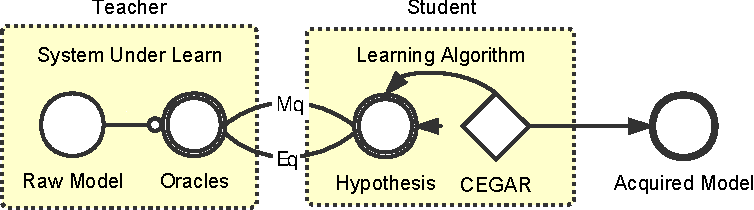
\includegraphics[width=.45\textwidth]{./images/actl.pdf}
  \end{center}
  \caption{Active Automata Learning}
  \label{fig:activelearning}
\end{figure}

Fig. \ref{fig:activelearning} shows the sketch of active learning, wherein:
\begin{itemize}
  \item[-] \emph{Teacher} and \emph{Student}: Active learning is an interactive process where
    students ask questions and teachers answer. Here learning algorithm plays the role of student.
  \item[-] \emph{Oracles} is an interface specifying which kind of questions can be answered by the
    teacher.
  \item[-] \emph{SUL} is an abbreviation of System Under Learn. In this paper, we take blackbox
    models as our SULs.
  \item[-] \emph{CEGAR} indicates Counter-Example Guided Abstraction
    Refinement\cite{DBLP:conf/cav/ClarkeGJLV00}. In active learning, we need counter-examples to
    guide us on further queries and cover the undistinguished states.
\end{itemize}

When applying active automata learning on some model, we assume that the model should be equivalent
to some \emph{Mealy machine}.
Such a model is encapsulated as a \emph{teacher} by the \emph{Oracle}, which handles
all communication with the model. The oracle also serves as a so-called \emph{Minimal Adequate
Teacher} \cite{DBLP:journals/iandc/Angluin87}
interface, which is responsible for two types of queries.

\begin{itemize}
  \item[-] \textbf{Membership Query} (hereinafter referred to as \emph{mq}) In grammar-learning
    \cite{DBLP:journals/iandc/Angluin87}, \emph{mq} checks if a word is a member of certain language
    defined by the given grammar. When it comes to
    automata learning, \emph{mq} is supposed to provide \emph{simulation results} for given input
    sequences.
  \item[-] \textbf{Equivalence Query} (hereinafter referred to as \emph{eq}) Given a hypothesis
    (usually constructed by the learning algorithm), \emph{eq} checks whether the hypothesis is
    equivalent to the system-under-learn and generates a counter-example if needed. 
\end{itemize}

These queries are given by \emph{learning algorithms}, or so-called \emph{students} in Fig.
\ref{fig:activelearning}. From the \emph{mq} results, a learning algorithm constructs a
\emph{hypothesis} and then check it with \emph{eq}. If counter-examples are found, we turn back and
repeat the hypothesis construction until the equivalence query returns \emph{true}.



%\subsection{Observation Table}
%\emph{Observation Tables}, proposed in \cite{DBLP:journals/iandc/Angluin87}, are used to describe
%hypothesises in form of Mealy machines.
%As mentioned before, Mealy machines are composed of \emph{states} and \emph{transitions}. However, in
%blackboxes, only \emph{input sequences} and their corresponding \emph{outputs} are observable. A
%natural idea is to use input sequences to indicate their corresponding states, and outputs to
%describe the edges.

%\begin{figure}[ht]
  %\begin{center}
    %\footnotesize
    %\begin{displaymath}
      %\begin{array}{l||ccccc}
        %\hline
        %& (a,\rread) & (\bot,\rread) & (a,\rnoread) & (\bot,\rnoread) & T \\
        %\hline\hline
        %\varepsilon & \rblock & \rblock & \rempty & \rempty & \rempty  \\
        %\hline
        %(a,\rread) & \rblock & \rblock & \rempty & \rempty & \rempty \\
        %(\bot,\rread) & \rblock & \rblock & \rempty & \rempty & \rempty \\
        %\rowcolor[gray]{.9}
        %(a,\rnoread) & \rblock & \rblock & \rblock & \rempty & \rempty \\
        %(\bot,\rnoread) & \rblock & \rblock & \rempty & \rempty & \rempty \\
        %T & \rblock & \rblock & \rempty & \rempty & \rempty  \\
        %\hline
      %\end{array}
    %\end{displaymath}
    %% 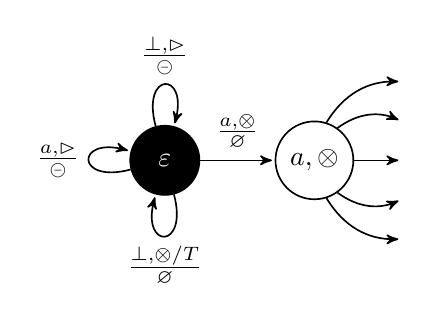
\begin{tikzpicture}[->,>=stealth',shorten >=1pt,auto,node distance=1.9cm,
  semithick]
  \tikzstyle{initial}=[fill=black, text=white]

  \node[initial,state] (Q0)               {$\varepsilon$};
  \node[state]         (Q1) [right of=Q0] {$a,\rnoread$};
  
  \path
  (Q0) edge [loop left]  node {$\frac{a,\rread}{\rblock}$} (Q0)
  (Q0) edge [loop above] node {$\frac{\bot,\rread}{\rblock}$} (Q0)
  (Q0) edge              node {$\frac{a,\rnoread}{\rempty}$} (Q1)
  (Q0) edge [loop below] node {$\frac{\bot,\rnoread/T}{\rempty}$} (Q0)
  (Q1) edge [bend left]  node {} (3,1)
  (Q1) edge [bend left]  node {} (3,0.5)
  (Q1) edge              node {} (3,0)
  (Q1) edge [bend right] node {} (3,-0.5)
  (Q1) edge [bend right] node {} (3,-1)
  ;
\end{tikzpicture}


  %\end{center}
  %\caption{Observation Table}
  %\label{fig:hypo}
%\end{figure}

%However, under such notations, there are \emph{infinite} number of states, among which most are
%duplicate.

%Now we use \emph{access sequence} to describe the states. Given an input sequence $s$, the access
%sequence $acc(s,D)$ of $s$ is defined as the shortest sequence in $\{s'\in\mathcal{I}^*|s'\sim_D
%s\}$\footnote{When there are multiple satisfying sequences with the same length, we use a certain tactic
%to pick up one from them determinstically.}.

%Formally, an observation table (see Fig. \ref{fig:hypo} as an example) is determined by a tuple $(S,D)$ where
%$S\subset\mathcal{I}^*$ is a set of the access sequences of states and $D\subset\mathcal{I}^*$
%is a set of suffixes. In such tables, columns are labelled with suffixes in $D$, and rows are
%labelled with input sequences. As shown in Fig. \ref{fig:hypo}, rows are divided into two parts. The upper
%part, labelled with access sequence $s\in S$, denotes the states covered in the current hypothesis.
%The lower part, labelled with sequences in $\{sa|s\in S,a\in\mathcal{I}\}\backslash S$ (representing
%any potentially unclosed transition) denotes all the transitions outside $s\in S$. A cell with row
%label $s$ and column label $d$ is filled with $mq(sd)$.

%An observation table $(S,D)$ is \emph{closed} if 
%\[
%\forall s\in S,a\in\mathcal{I}.\exists s'\in S. sa\sim_D s'
%\]

%From a closed observation table $obs$, we can construct a hypothetical Mealy machine $\mathcal{H}=\langle
%S,s_0,\mathcal{I},\mathcal{O},\delta,\lambda\rangle$ in a straight-forward way:
%\begin{itemize}
  %\item[-] Every state in $S$ corresponds to an input sequence in $obs.S$
  %\item[-] $s_0$ corresponds to the empty sequence $\varepsilon$
    
    %\emph{(we use input sequences to indicate their corresponding states in following parts)}
  %\item[-] $\delta(s,a)=mq(sa)$
  %\item[-] $\lambda(s,a)=acc(sa,obs.D)$. Since $obs$ is closed, we always have $\lambda(s,a)\in S$.
%\end{itemize}

%Algorithm \ref{alg:buildtable} shows how to build a closed observation table.

%\begin{algorithm} 
  %\caption{EncloseTable} 
  %\label{alg:buildtable}
  %\small
  %\KwIn{An oracle interface $mq$, An input actions $\mathcal{I}$, An observation table $obs$}
  %\KwOut{A closed observation table $obs'$} 
  %\Repeat{$unclosed=\varnothing$}
  %{
    %$next=\{st|\forall s\in obs.S,\forall t\in \mathcal{I}\}\backslash obs.S$\;
    %$unclosed=\{seq\in next|\forall a\in obs.S, seq \not\sim_{obs.D} a\}$\;
    %$obs'.S$ = $obs.S\cup unclosed$\;
    %$obs'.D$ = $obs.D$\;
  %}
  %\Return $obs'$\; 
%\end{algorithm}

%Taking a 2-Timer channel as an example, we now illustrate how this algorithm works. 
%We assume that the source end of this 2-Timer channel is $A$, the sink end is $B$, and the alphabet
%is $\{a\}$. We briefly denote $\{A\mapsto a,B\mapsto \rnoread\}$ and other input/output actions in form of
%$(a,\rnoread)$.

%Firstly, $obs.S$ is initialized with the initial state (denoted by $\varepsilon$), and $obs.D$ is
%initialized with all one-step suffixes.
%Then we explore all the access sequences in $obs.S$ and calculate its successors. Here
%$unclosed$ consists of access sequences that has no equivalent sequence in $obs.S$. 
%For example, Fig. \ref{fig:hypo} shows the $obs$ of a 2-Timer channel after the first
%iteration. The five successors of $\varepsilon$ are presented at the bottom of the table, where
%four are equivalent with $\varepsilon$ but $(a,\rnoread)$ is not. Therefore, we take $(a,\rnoread)$ as a
%brand-new state and all of its successors need further exploration. 


%In the second iteration, we explore the successors of $(a,\rnoread)$. Fortunately, now every
%successor has an equivalence sequence in $obs.S$, \emph{i.e.}, itself. Consequently, the algorithm terminates
%with a closed hypothesis where all the unclosed edges turn into
%self-loop.

%%\begin{figure}[ht]
  %%\begin{center}
    %%\begin{displaymath}
      %%\begin{array}{l||ccccc||c}
        %%\hline
        %%& (a,\rread) & (\bot,\rread) & (a,\rnoread) & (\bot,\rnoread) & T & acc\\
        %%\hline\hline
        %%\varepsilon & \rblock & \rblock & \rempty & \rempty & \rempty & \varepsilon \\
        %%(a,\rnoread) & \rblock & \rblock & \rblock & \rempty & \rempty & (a,\rnoread) \\
        %%\hline
        %%(a,\rread) & \rblock & \rblock & \rempty & \rempty & \rempty & \varepsilon\\
        %%(\bot,\rread) & \rblock & \rblock & \rempty & \rempty & \rempty & \varepsilon \\
        %%(\bot,\rnoread) & \rblock & \rblock & \rempty & \rempty & \rempty & \varepsilon \\
        %%T & \rblock & \rblock & \rempty & \rempty & \rempty & \varepsilon \\
        %%(a,\rnoread),(a,\rread) & \rblock & \rblock & \rblock & \rempty & \rempty & (a,\rnoread) \\
        %%(a,\rnoread),(\bot,\rread) & \rblock & \rblock & \rblock & \rempty & \rempty & (a,\rnoread) \\
        %%(a,\rnoread),(a,\rnoread) & \rblock & \rblock & \rblock & \rempty & \rempty & (a,\rnoread) \\
        %%(a,\rnoread),(\bot,\rnoread) & \rblock & \rblock & \rblock & \rempty & \rempty &
        %%(a,\rnoread) \\
        %%(a,\rnoread),T & \rblock & \rblock & \rblock & \rempty & \rempty & (a,\rnoread) \\
        %%\hline
      %%\end{array}
    %%\end{displaymath}
  %%\end{center}
  %%\caption{A Closed Version of Fig. \ref{fig:hypo}}
  %%\label{fig:hypo2}
%%\end{figure}

%\subsection{Counter Examples' Analysis} 
%Apparently, the closed hypothesis presented in Fig. \ref{fig:hypo2} is different with the 2-Timer
%channel. It's easy to find a counter-example $s_0=(a,\rnoread),T,T,(\bot,\rread)$ where $mq(s_0)=a$ while
%according to the hypothesis, the result should be $\rempty$. In this section, we show how to
%find and analyze counter-examples using the method in \cite{DBLP:conf/sfm/SteffenHM11}. 

%Firstly, we give a formal definition of \emph{counter examples}. With an observation table $obs$ and
%a sequence $s$, we use $hq(obs,s)$ to denote the execution result of its corresponding hypothesis
%$\mathcal{H}$ under the input sequence
%$s$. Obviously we have $hq(obs,s) = mq(acc(s')a)$ where $s=s'a,a\in\mathcal{I}$.

%\begin{definition}[Counter Example]
  %an input sequence $s$ is a counter example of $obs$ iff $mq(s)\neq hq(obs,s)$.
%\end{definition}

%Now we consider the reason that leads to existance of counter examples. Since
%the suffix set $D$ is used to distinguish states, the existance of counter-examples
%shows that the current suffix set $D$ is not powerful enough to recognize the uncovered states in
%$next$ (see Algorithm \ref{alg:buildtable}).

%For a counter example $s$, we need a new Suffix$(s,obs)$ to distinguish the uncovered state
%represented by $s$, which is defined as the longest sequence in
%\[
%\{d\in\mathcal{I}^+|s=s'd, mq(acc(s',obs.D)d)\neq mq(s)\}
%\]
%After appending Suffix$(s,obs)$ to $D$, it's obvious that at least one uncovered state will be found.

\subsection{L* Algorithm}
The whole L* algorithm can be briefly concluded as follows. In this algorithm,
\begin{itemize}
  \item \emph{observation table} is a widely-used data structure to describe the hypothesis.
\end{itemize}
Please refer to \cite{DBLP:conf/sfm/SteffenHM11, DBLP:journals/iandc/Angluin87} for further details.
\begin{algorithm} 
  \caption{L*} 
  \label{alg:lstar}
  \KwIn{Oracle interfaces $mq,eq$, Input actions $\mathcal{I}$}
  \KwOut{Observation table $obs$} 
  $obs.S$ initialized as empty\;
  $obs.D$ initialized as $\{[i]|i\in\mathcal{I}\}$\;
  \Repeat{$ce=true$}{
    $obs$ = EncloseHypothesis($mq$, $\mathcal{I}$, $obs$)\;
    $ce=eq(obs)$\;
    \If {$ce\neq true$} {
      $obs.D$.append(Suffix$(ce, obs)$)\;
    }
  }
  \Return $obs$\; 
\end{algorithm}

The L* algorithm takes a set of input actions $\mathcal{I}$ and a oracle interface (which plays the
role of SUL) as its parameters. And it returns a so-called \emph{observation table} as the final
hypothesis. (Observation table is a widely-used data structure, which can represent a Mealy machine
by its external observation.)
In each iteration, the algorithm will:
\begin{enumerate}
  \item \emph{Enclose the hypothesis.} Active learning is very similar to a breadth-first-search
    process on an unknown Mealy machine. At first, only the initial state is visible to us. We then
    explore different input actions and check if they can lead to some state that is already known.
    If every edge targets to an explored state, we will say that the hypothesis is \emph{closed}.
  \item \emph{Equivalence checking.} After the hypothesis is enclosed, we need to check if the
    current hypothesis is equivalent to the real model. Such $eq$ operation returns a
    \emph{true} if they are equivalent, or a counter-example if not.
  \item \emph{Counter-example Analysis.}  
\end{enumerate}


\section{Experiments}  
\label{sec:experiment}

Both \emph{Reo Coordination Models} and \emph{Adapted L* Algorithm} are implemented in
Golang. With a CSP-style\cite{DBLP:books/ph/Hoare85} cocurrency model, the Google-production language
\texttt{Golang} shares quite a few similar ideas with Reo, and in turn makes our implementation much
more natural.

All the following experiments are coded under Golang \emph{1.2.1} and executed on a laptop with 8GB
of RAM and a Core i7-3630 CPU. The source code is available at \cite{reo-learn-github}.

\subsection{Case Study}
A simple example of timed connector is presented to show how L* works.
\begin{figure}[ht]
  \begin{center}
    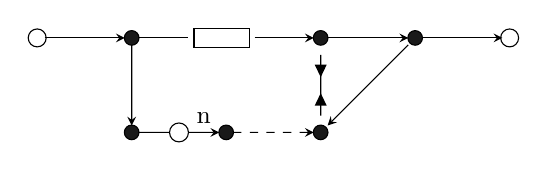
\begin{tikzpicture}[scale=1.2]
  \tikzset{every node} = [font=\small]

  \ionode{(P-A)}{(0,0)}{}
  \ionode{(P-B)}{(5,0)}{}
  \mixednode{(P-C)}{(1,0)}{}
  \mixednode{(P-D)}{(3,0)}{}
  \mixednode{(P-E)}{(4,0)}{}
  \mixednode{(P-F)}{(1,-1)}{}
  \mixednode{(P-G)}{(2,-1)}{}
  \mixednode{(P-H)}{(3,-1)}{}

  \fifoe{(P-C)}{(P-D)}{}
  \syncdrain{(P-D)}{(P-H)}{}
  \sync{(P-A)}{(P-C)}{}
  \sync{(P-C)}{(P-F)}{}
  \sync{(P-D)}{(P-E)}{}
  \sync{(P-E)}{(P-B)}{}
  \sync{(P-E)}{(P-H)}{}
  \lossysync{(P-G)}{(P-H)}{}

  \timer{(P-F)}{(P-G)}{node [above] {n}}

\end{tikzpicture}

  \end{center}
  \caption{Expiring FIFO1 (ExpFIFO1)}
  \label{fig:expfifo}
\end{figure}

Informally speaking, an expiring FIFO1 with \emph{timeout} $n$ is able to accept a data item
and stored it in the buffer cell for $n$ time units. If a read operation on $B$ is performed within
$n$ time units, it will obtain the data item successfully and clear the buffer. Otherwise, the data
item would be dropped if no read operation comes within $n$ time units.

\begin{figure}[ht]
  \begin{center}
    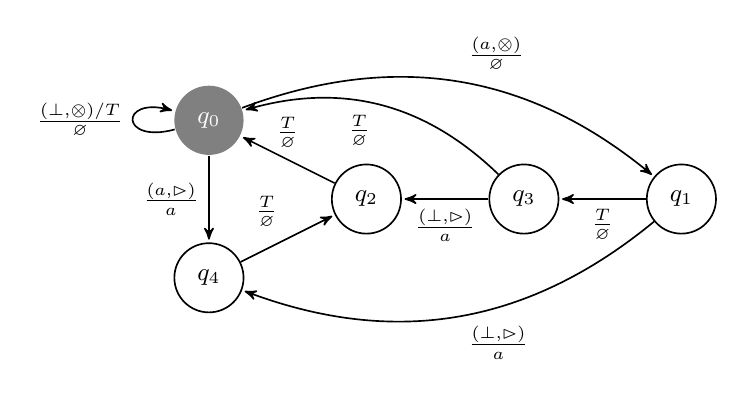
\begin{tikzpicture}[->,>=stealth',shorten >=1pt,auto,node distance=1.9cm,
  semithick]
  \tikzstyle{initial}=[fill=gray,text=white]
  \tikzstyle{every node}=[font=\small]
  \tikzstyle{nodraw}=[draw=none]

  \node[initial,state, nodraw] (Q0) at (0,1)   {$q_0$};
  \node[state]         (Q1) at (6,0)   {$q_1$};
  \node[state]         (Q2) at (2,0)  {$q_2$};
  \node[state]         (Q3) at (4,0)   {$q_3$};
  \node[state]         (Q4) at (0,-1)  {$q_4$};
  
  \path
  (Q0) edge [bend left]  node         {$\frac{(a,\rnoread)}{\rempty}$} (Q1)
  (Q0) edge              node [left]  {$\frac{(a,\rread)}{a}$} (Q4)
  (Q0) edge [loop left]  node         {$\frac{(\bot,\rnoread)/T}{\rempty}$} (Q0)
  (Q1) edge              node         {$\frac{T}{\rempty}$} (Q3)
  (Q1) edge [bend left]  node         {$\frac{(\bot,\rread)}{a}$} (Q4)
  (Q2) edge              node [above] {$\frac{T}{\rempty}$} (Q0)
  (Q3) edge              node         {$\frac{(\bot,\rread)}{a}$} (Q2)
  (Q3) edge [bend right] node         {$\frac{T}{\rempty}$} (Q0)
  (Q4) edge              node         {$\frac{T}{\rempty}$} (Q2)
  ;
\end{tikzpicture}


  \end{center}
  \caption{Learn Result of The ExpFIFO1 where $n=2,\Sigma=\{a\}$}
  \label{fig:expfifosemantics}
\end{figure}

Fig. \ref{fig:expfifosemantics} shows the learning result of this example where $n=2$ and
$\Sigma=\{a\}$.
To simplify the graph, we ignore all the trivial transitions $\frac{(\bot,\rnoread)}{\rempty}$
and block transitions. More details of this case can be found in our \emph{github repo}.

\subsection{Performance Optimization}
As a well-known learning algorithm, L* has proved its efficiency in models without time.
However, when dealing with timed connectors, the algorithm failed to meet our expectation.

\begin{table}[ht]
  \renewcommand{\arraystretch}{1.3}
  \caption{Time-Cost Analysis}
  \label{tabel:timecost}
  \centering
  \begin{tabular}{l||rrr}
    \hline
    & FIFO1 & Alternator & Gate \\
    \hline\hline
    Membership Query(s) & 41.571 & 126.468 & 169.161 \\
    Hypothesis Query(s) & 0.001 & 0.003 & 0.004 \\
    Total Time(s) & 41.715 & 165.114 & 247.098 \\
    Membership Query(\%) & 99.6 & 76.6 & 68.5 \\
    \hline
  \end{tabular}
\end{table}

As shown in Table \ref{tabel:timecost}, time consumption mainly comes from membership queries.
With time involved, every single membership query takes a lot of time inevitably.
After reviewing our algorithm, we found that simulations on similar sequences were invoked frequently:

\begin{itemize}
  \item When constructing observation tables, there are lots of redundant calls to membership
    queries. For example, a sequence with prefix `aa' and suffix `b' is exactly same as another one
    with prefix `a' and suffix `ab'.
  \item Simulation on Mealy machines can provide multi-step outputs.  Consequently, if we have
    simulated an `abc' sequence, it's useless to perform simulation on an `ab' sequence again.
\end{itemize}

If previous simulation results are stored in a well-maintained cache, the time-cost in
simulation process could be reduced signficiantly. In this work, we use a multiway tree to buffer
these results.

\begin{table}[ht]
  \renewcommand{\arraystretch}{1.3}
  \caption{Reduction of Membership Queries}
  \label{tabel:cacheoptimization}
  \centering
  \begin{tabular}{l||rrr}
    \hline
    & FIFO & Alternator & Gate \\
    \hline\hline
    Original Algorithm & 93 & 880 & 1034 \\
    Cached Algorithm & 90 & 725 & 707 \\
    Reduction Rate & 3.2\% & 21.4\% & 31.6\% \\
    \hline
  \end{tabular}
\end{table}

With the help of cache technique, we have made considerable reduction on the calls of membership queries. The results
can be found in Table \ref{tabel:cacheoptimization}.

\section{Conclusion and Fu ture Work}
In this paper, we come up with an approach to extract timed connectors from blackbox
implementations. We propose \emph{parameterized Mealy machine} to describe the behavior of Reo
connectors. Then we define the product operator and link operator, which can be used to
construct complex connectors from simpler ones.
Besides, we show how PMMs behave as the bridge between Reo connectors and concrete Mealy
machines with timed action T provided. 

We also adapt the well-known active learning algorithm L* to deal with time domain.
% When time is taken into consideration, the original L* algorithm run into a performance bottleneck.
By a tree-style cache, we make significant reduction on membership queries and, in turn,
improve the performance of learning algorithm. As a by-product, we also encapsulate the Reo
connector as a distributable package which could contribute to concurrent programming.

Our future work mainly focuses on better support of dense time. To describe dense
time behavior, the Mealy machine model needs a lot of changes instead of a simple T action. Besides,
we will also try to improve our algorithm to handle non-deterministic behavior. This is not a brand
new topic \cite{DBLP:conf/isola/VolpatoT14}, but we believe that there is still room for
improvement.  

\section*{Acknowledgments}
The work was partially supported by the National Natural Science Foundation of China under grant no.
61202069, 61272160 and 61532019.
\bibliographystyle{abbrv}
\bibliography{bib}

\end{document}
